\documentclass{article}
\usepackage[backend=biber,citestyle=ieee]{biblatex}
\usepackage[english]{babel}
%\usepackage[swedish]{babel}
\usepackage{graphicx}
\usepackage{csquotes}
\usepackage{float}
\usepackage{url}
\usepackage[hidelinks]{hyperref}
\usepackage{siunitx}
\usepackage{datetime}
\usepackage[title]{appendix}
\usepackage[font={small},margin={1cm}]{caption}
\usepackage{titlesec}
\usepackage{enumitem}
\usepackage{amsmath}
\usepackage{fancyhdr}   %page header
\usepackage[margin=1in]{geometry}

\pagestyle{fancy}
\fancyhf{}

\cfoot{Page \thepage}

\usepackage[parfill]{parskip} %Line skip between paragraphs instead of indent

\usepackage{xcolor}
\usepackage{listings}   %code section 



\newcommand{\getauthor}{Eric Johansson (erjo2002@student.miun.se)\\Can Kupeli (caku2002@student.miun.se) \\Samuel Greenberg (sagr1908@student.miun.se)} %Author
\newcommand{\gettitle}{Laboration 1 \\Equations and Differencial Methods} %Title
\newcommand{\getcourse}{(MA069G, Mathematical Modelling 6hp)} %Course
\newcommand{\getsupervisor}{Cornelia Schiebold\\Magnus Eriksson\\Suprokash Hazra}


\begin{document}
  \begin{titlepage}
	\begin{center}
		\vspace*{1cm}

		
\includegraphics[width=0.8\textwidth]{imgs/msu.png}\\[0.5cm]
		\Large
		Institution of Information Systems and -Technology (IST)\\[1cm]
		\Huge
		\rule{\textwidth}{1px}
		\textbf{\gettitle}
		\rule[0.5cm]{\textwidth}{1px}

		\large
		\getcourse{}
		\vspace{1cm}

        \Large
		\textbf{\getauthor}\\

		\vfill


		\vspace{0.8cm}

		\small
		\today \\
		\Large
		\textbf{Supervisor:}\\
		\getsupervisor{}

	\end{center}
\end{titlepage}
\tableofcontents
\newpage

  
\section{}

\begin{figure}[h]
	\centering
	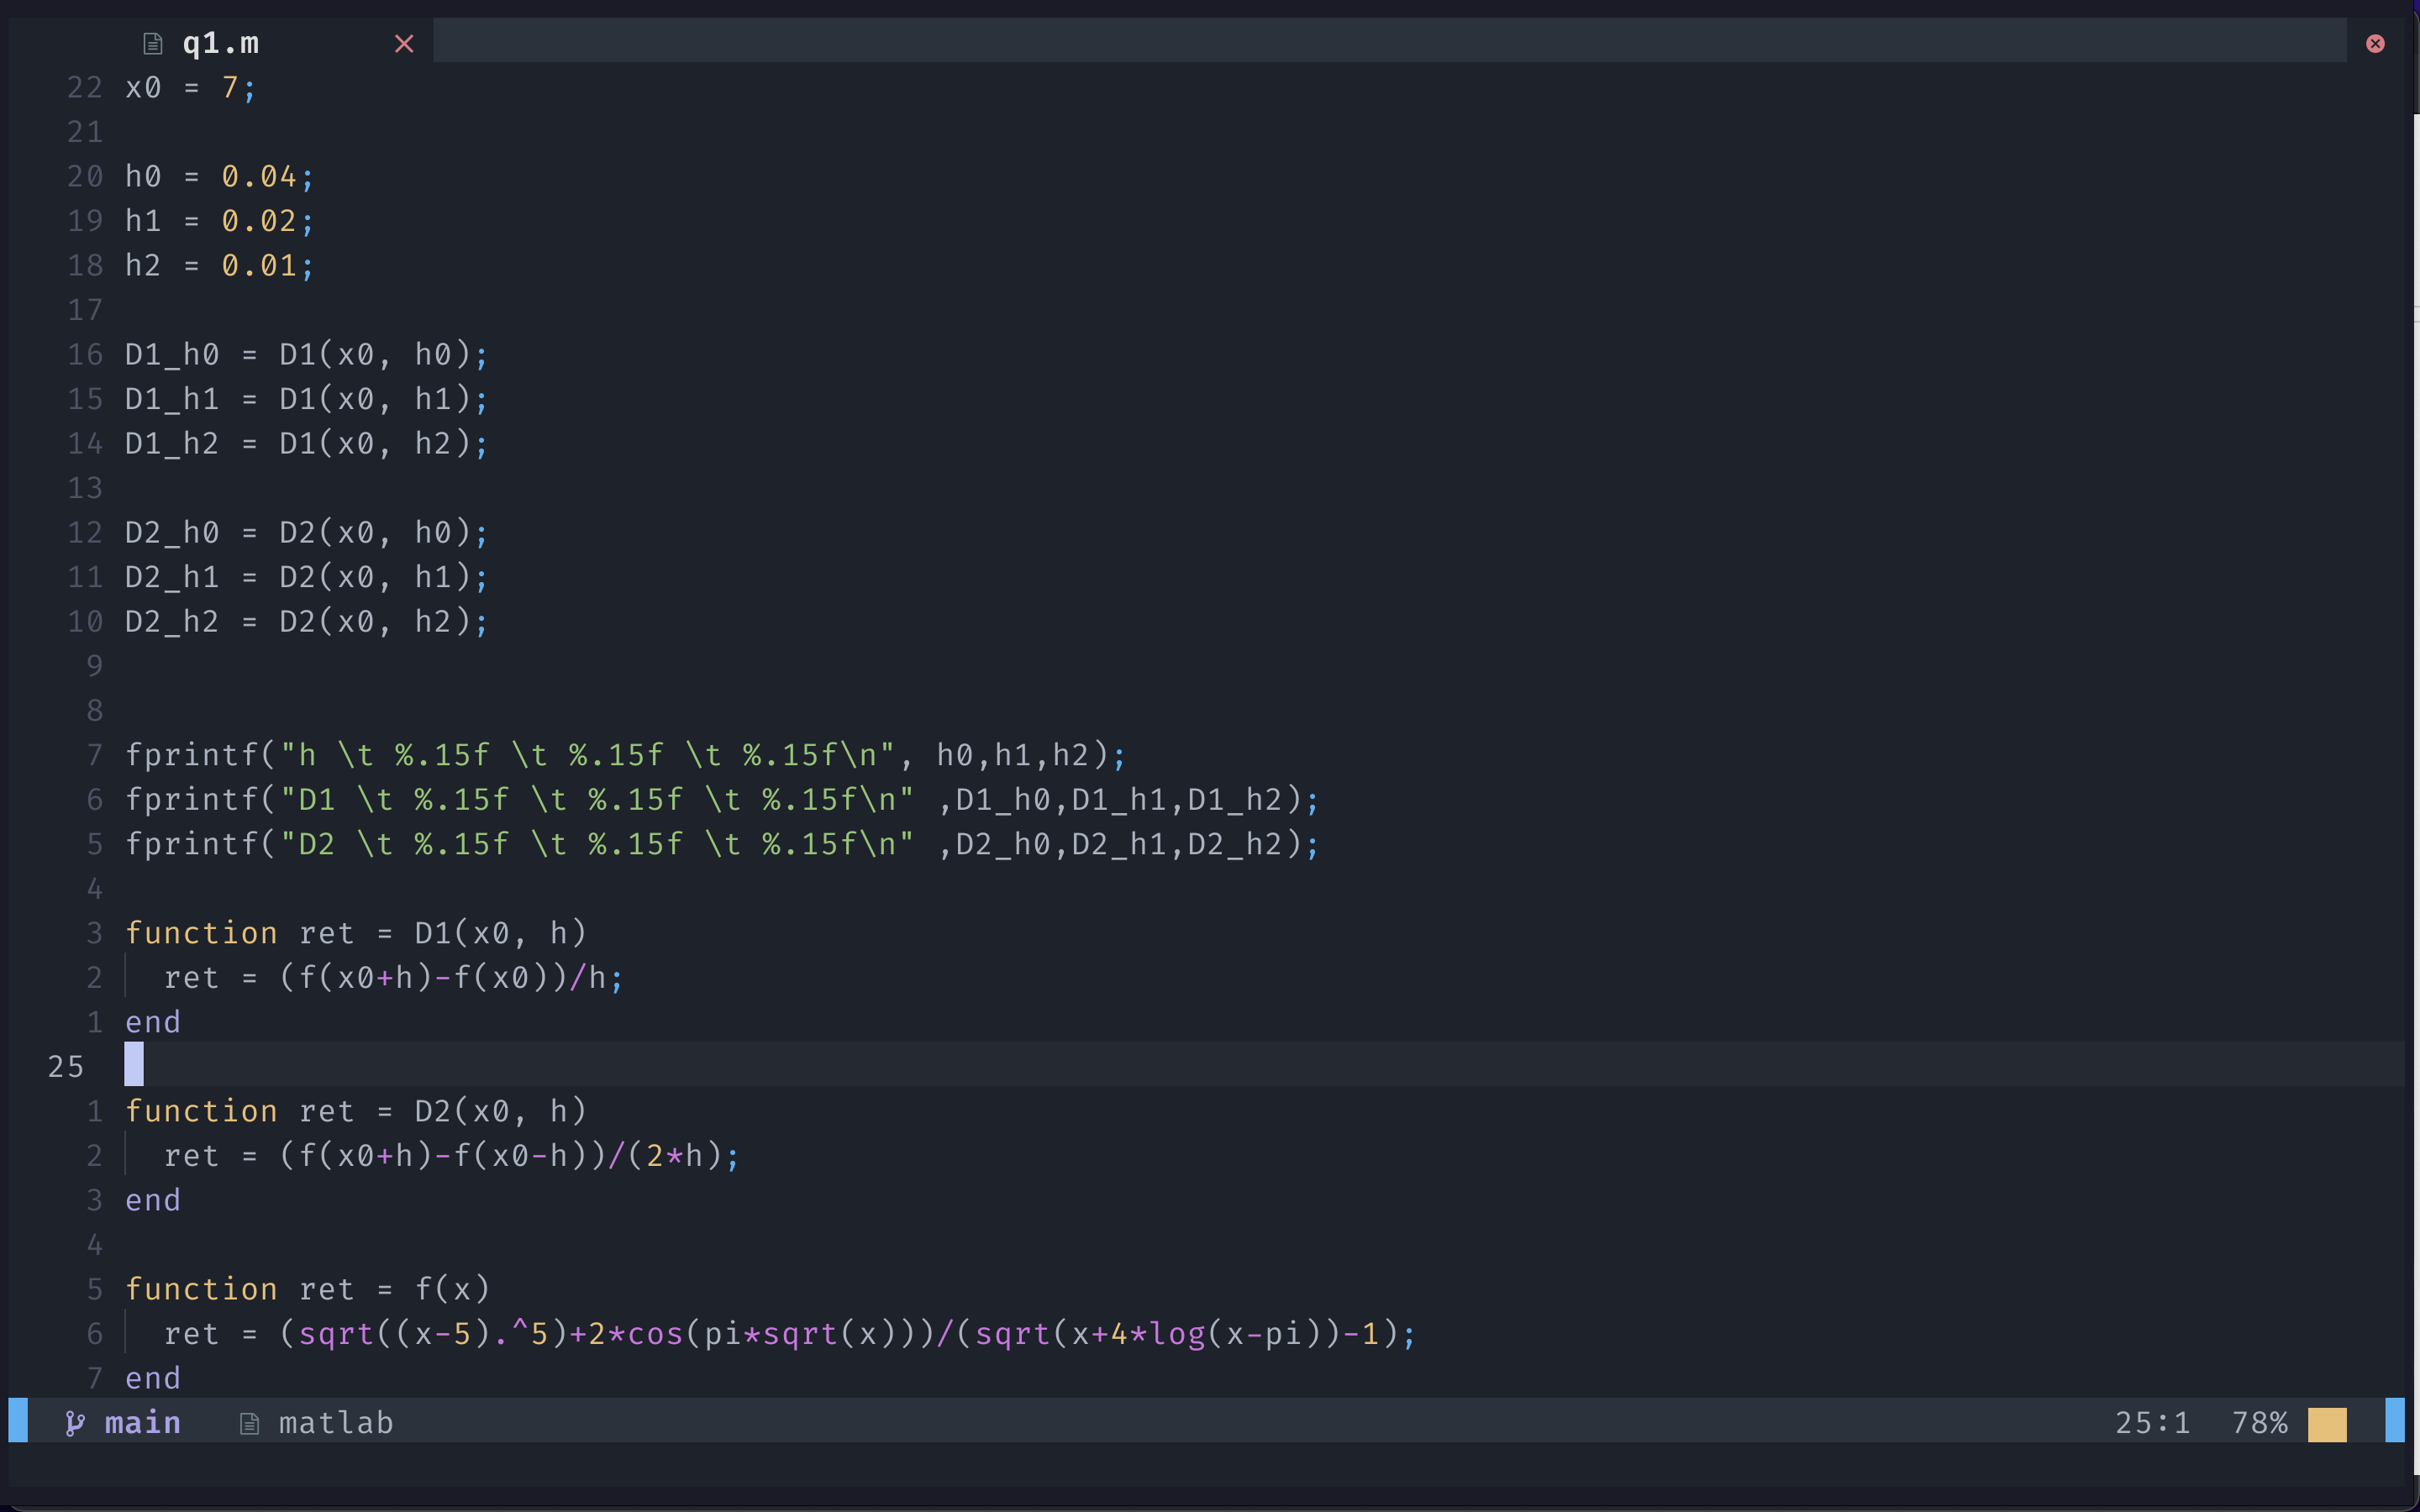
\includegraphics[width=\textwidth]{imgs/q1_code.png}
	\caption{Code for question one}
	\label{fig:q1_code}
\end{figure}

\begin{figure}[h]
	\centering
	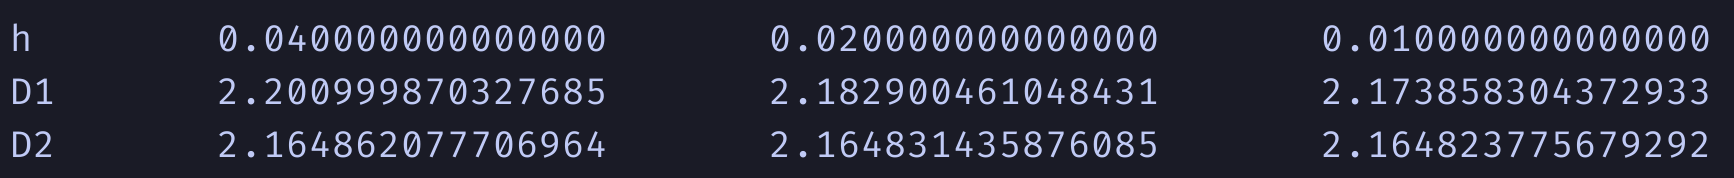
\includegraphics[width=\textwidth]{imgs/q1_results.png}
	\caption{Output for question one}
	\label{fig:q1_results}
\end{figure}

These results show that D2, the central difference, is closer to the actual value of $f^\prime(x_0)$. This is because the method has a
truncation error of $O(h^2)$, whereas the forward difference only has $O(h)$. $O(h^{2})$ is more prefferable to $O(h)$ because when $\lim_{h \to 0}$ the term $O(h^{2})$ converges towards $0$ faster than $O(h)$.

\newpage
\section{}
\begin{figure}[H]
	\centering
	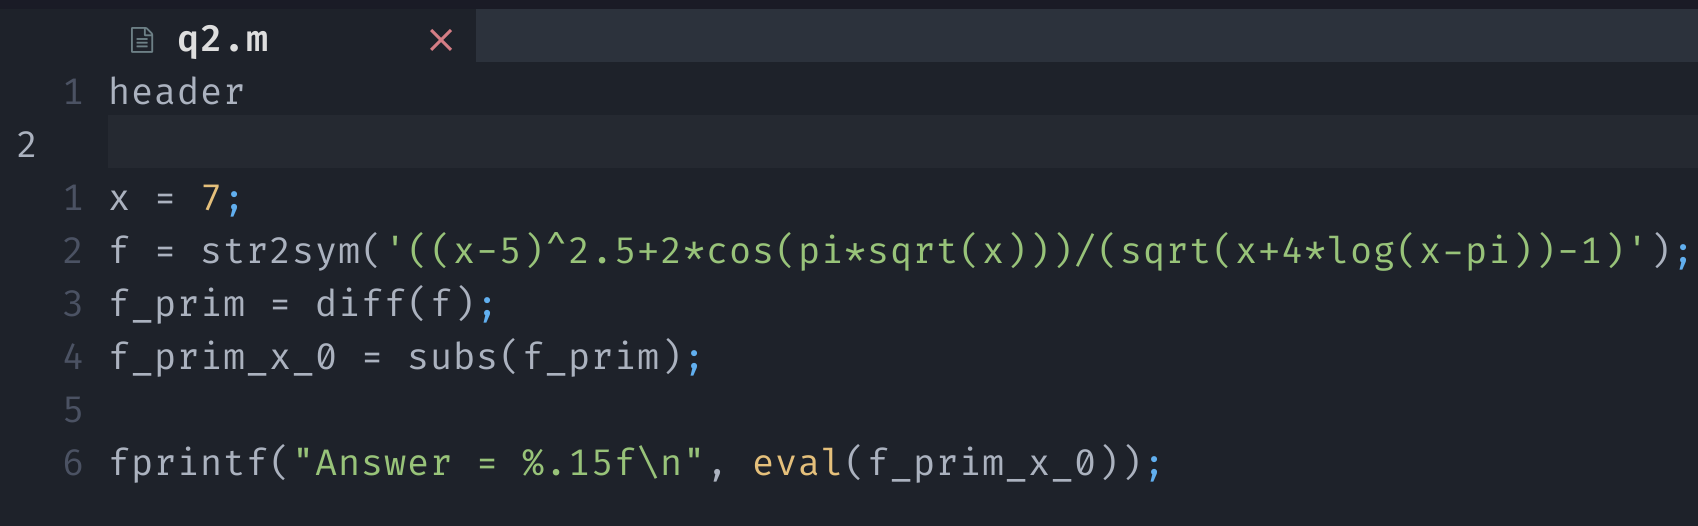
\includegraphics[width=\textwidth{}]{imgs/q2_code.png}
	\caption{Code for question 2}
	\label{fig:q2_code}
\end{figure}

\begin{figure}[H]
	\centering
	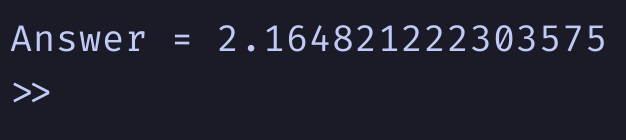
\includegraphics[width=0.5\textwidth]{imgs/q2_results.png}
	\caption{Results for question 2}
	\label{fig:q2_results}
\end{figure}
The outputted value, shown in figure 4, is equal to the actual value of the functions derivative, with a precision of at least 15 decimal places.

\newpage
\section{}
\begin{figure}[H]
	\centering
	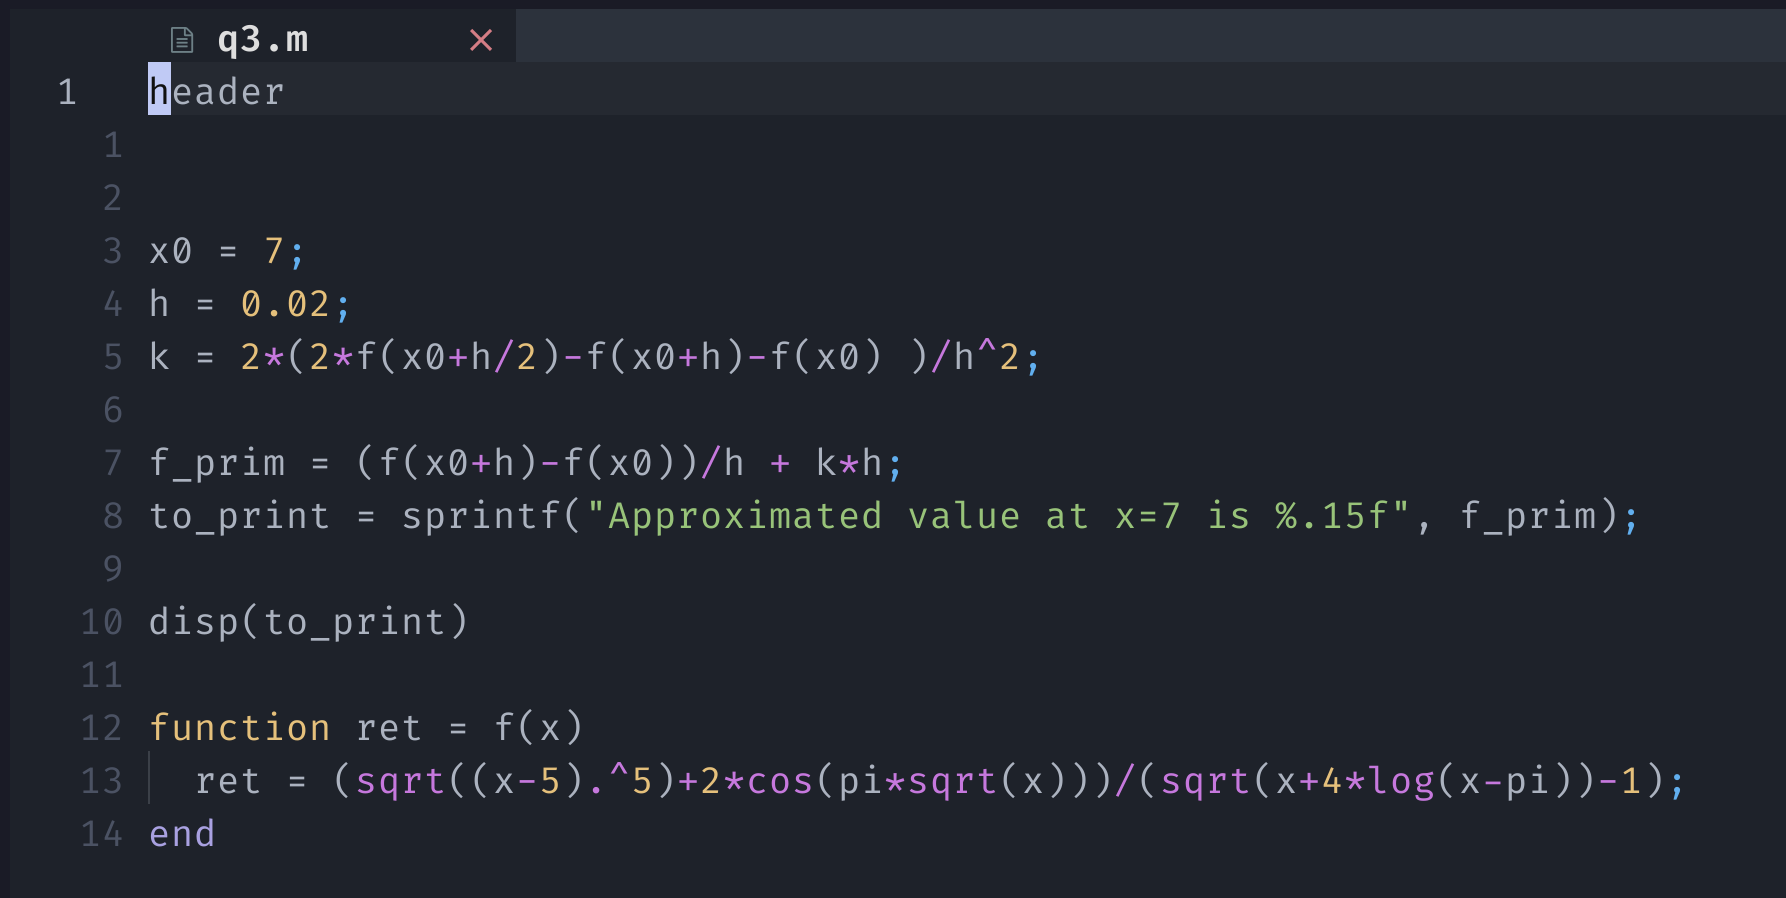
\includegraphics[width=0.8\textwidth]{imgs/q3_code.png}
	\caption{Code for question 3}
	\label{fig:q3_code}
\end{figure}

\begin{figure}[H]
	\centering
	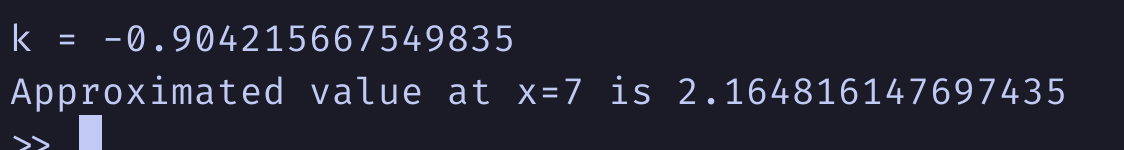
\includegraphics[width=0.8\textwidth]{imgs/q3_results.png}
	\caption{Results for question 3}
	\label{fig:q3_result}
\end{figure}
Due to the given $h$-value being relatively far from $0$, the approximation of $k$ and consequently the derivative, were a few deiciamls off from the correct value.

\newpage
\section{}
\begin{figure}[H]
	\centering
	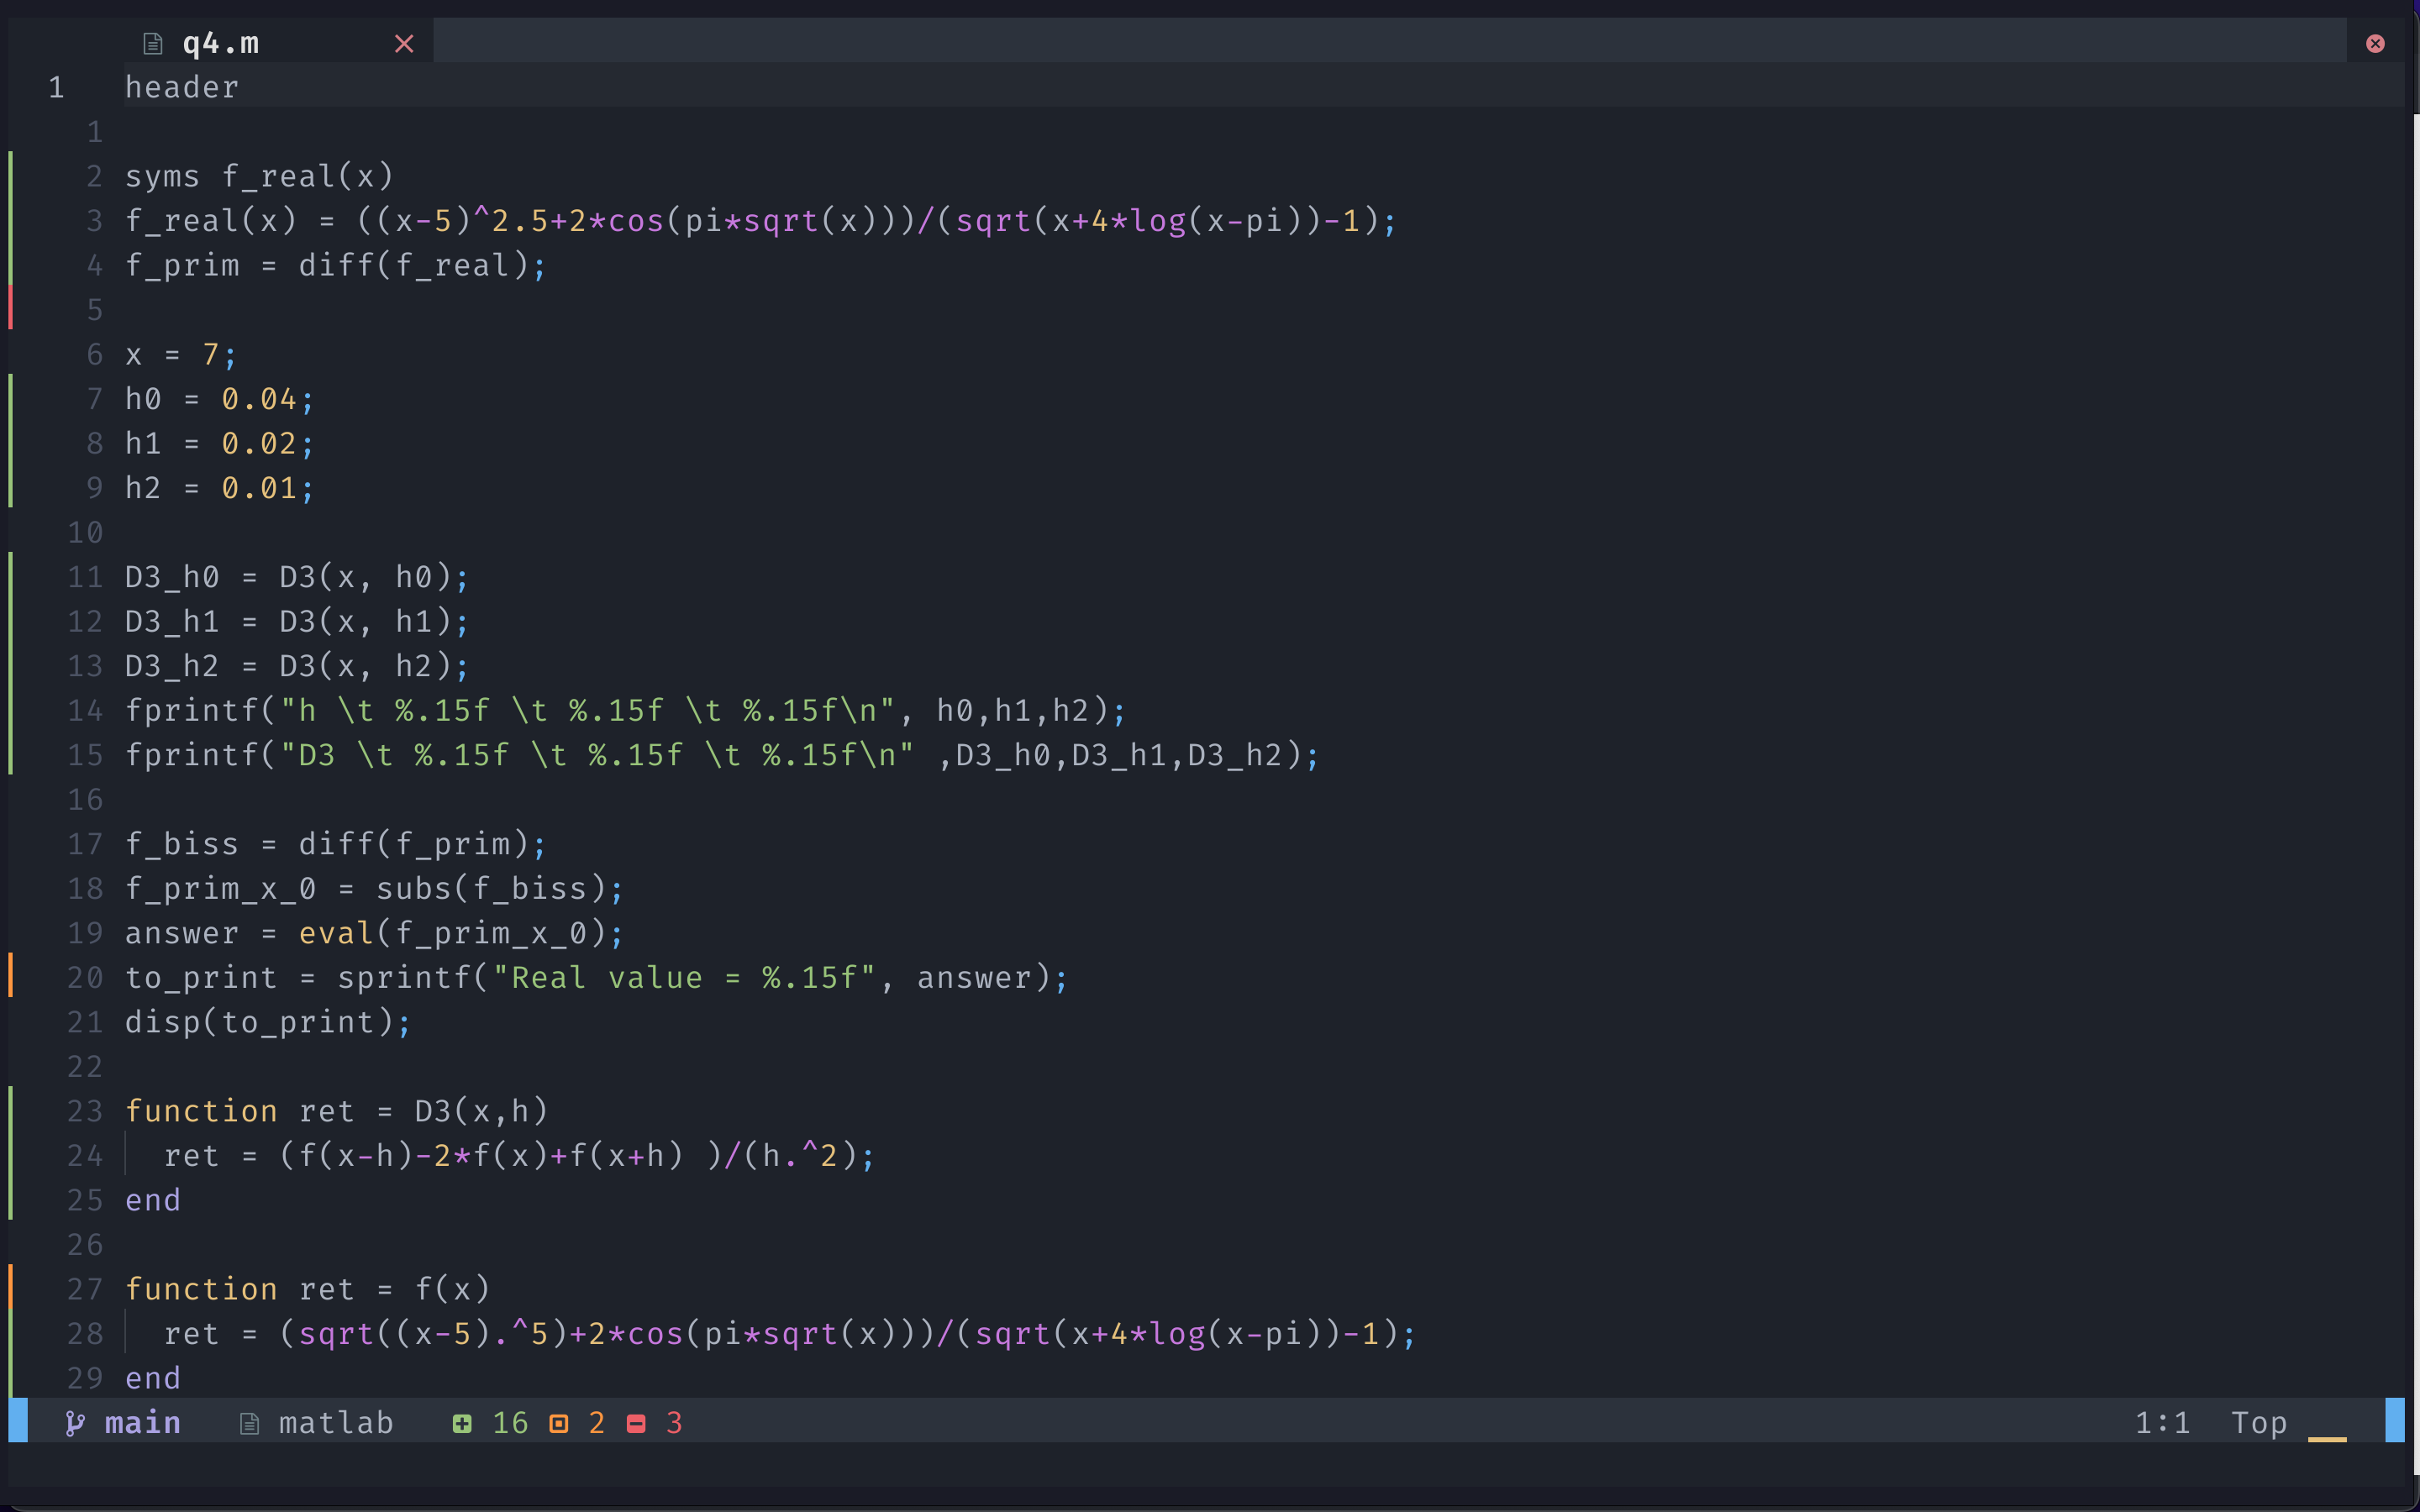
\includegraphics[width=\textwidth]{imgs/q4_code.png}
	\caption{Code for question 4}
	\label{fig:q4_code}
\end{figure}

\begin{figure}[H]
	\centering
	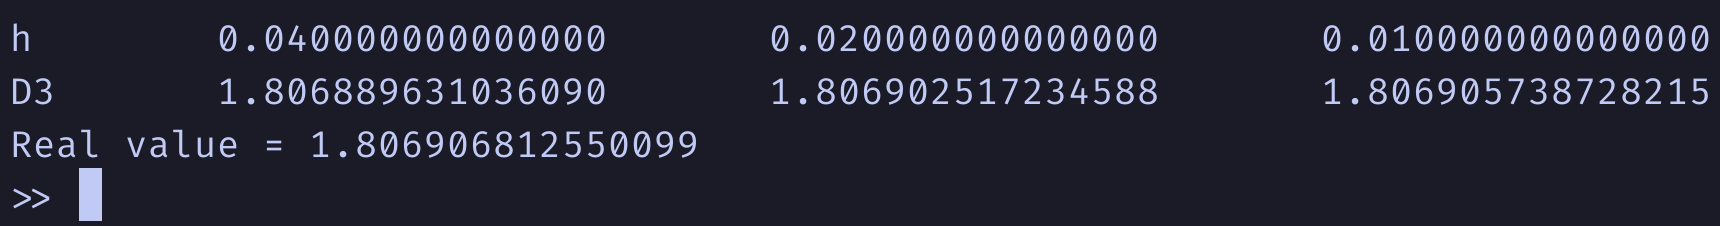
\includegraphics[width=\textwidth]{imgs/q4_results.png}
	\caption{Results for question 4}
	\label{fig:q4_result}
\end{figure}

\newpage
\section{}

\begin{figure}[H]
	\centering
	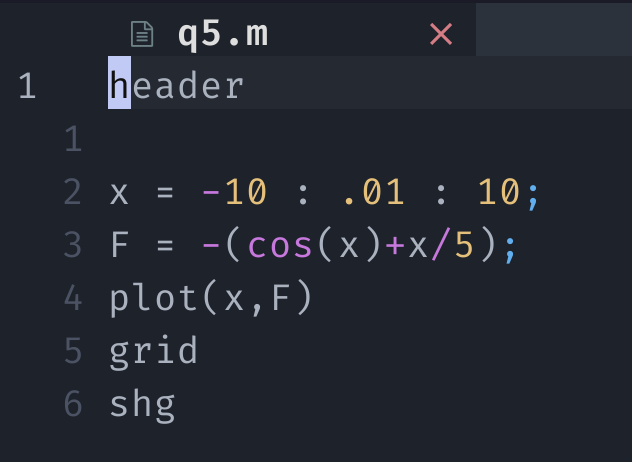
\includegraphics[width=0.5\textwidth]{imgs/q5_code.png}
	\caption{Code for question 5}
	\label{fig:q5_code}
\end{figure}

\begin{figure}[H]
	\centering
	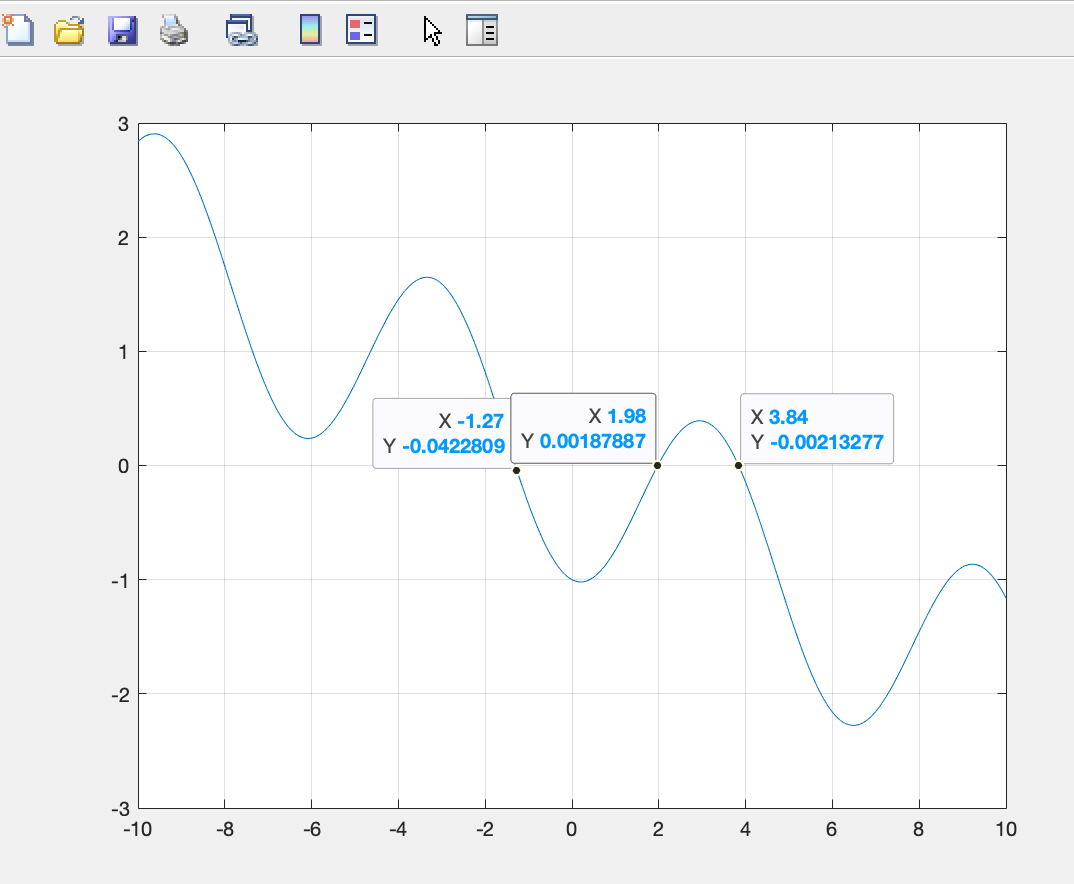
\includegraphics[width=0.8\textwidth]{imgs/q5_results.png}
	\caption{Results for question 5}
	\label{fig:q5_result}
\end{figure}

\newpage
\section{}
\begin{figure}[H]
	\centering
	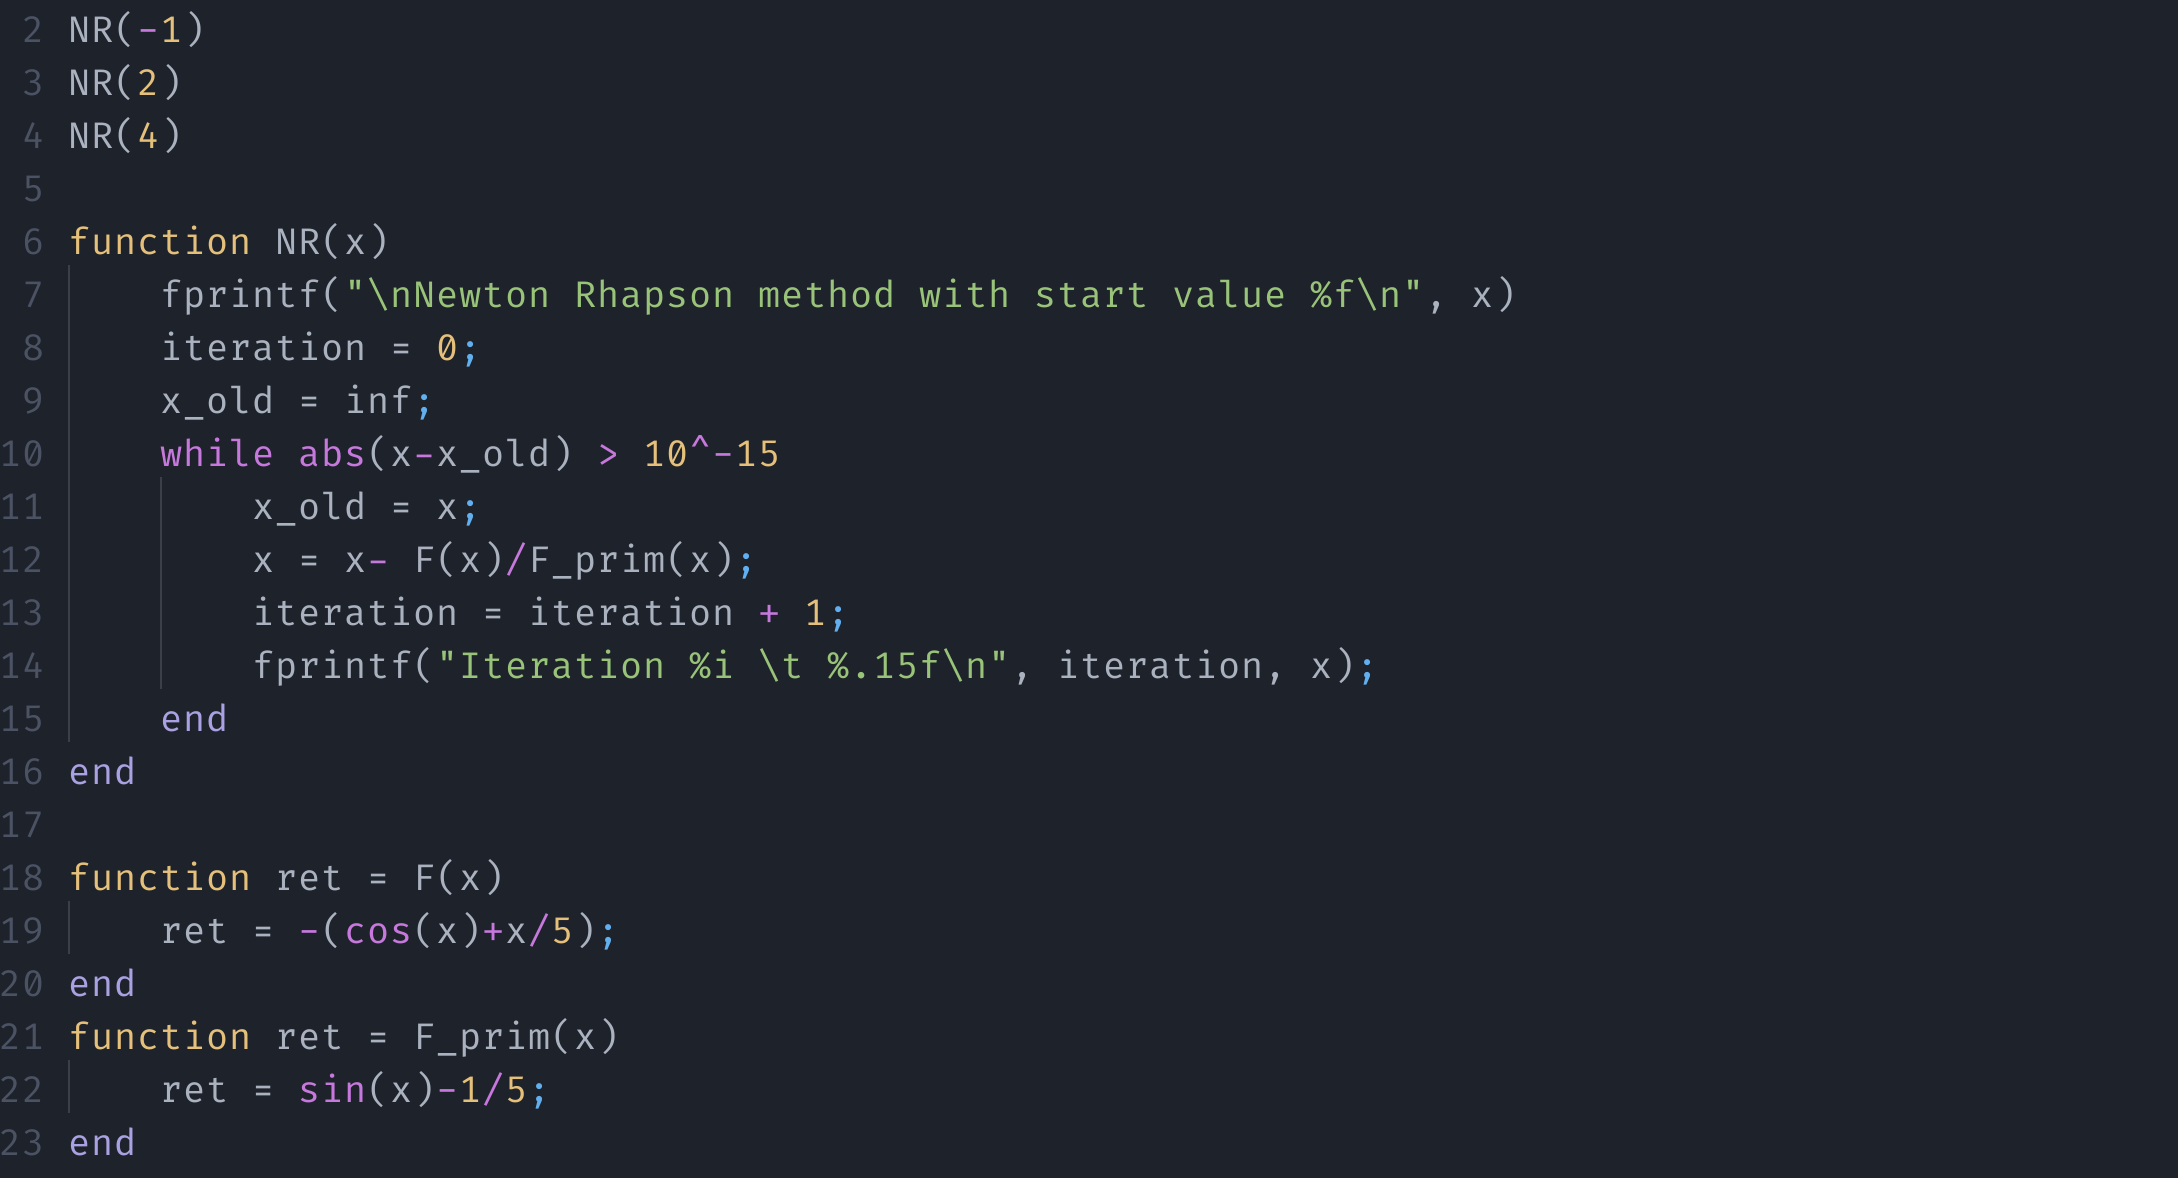
\includegraphics[width=0.8\textwidth]{imgs/q6_code.png}
	\caption{Code for question 6}
	\label{fig:q6_code}
\end{figure}

\begin{figure}[H]
	\centering
	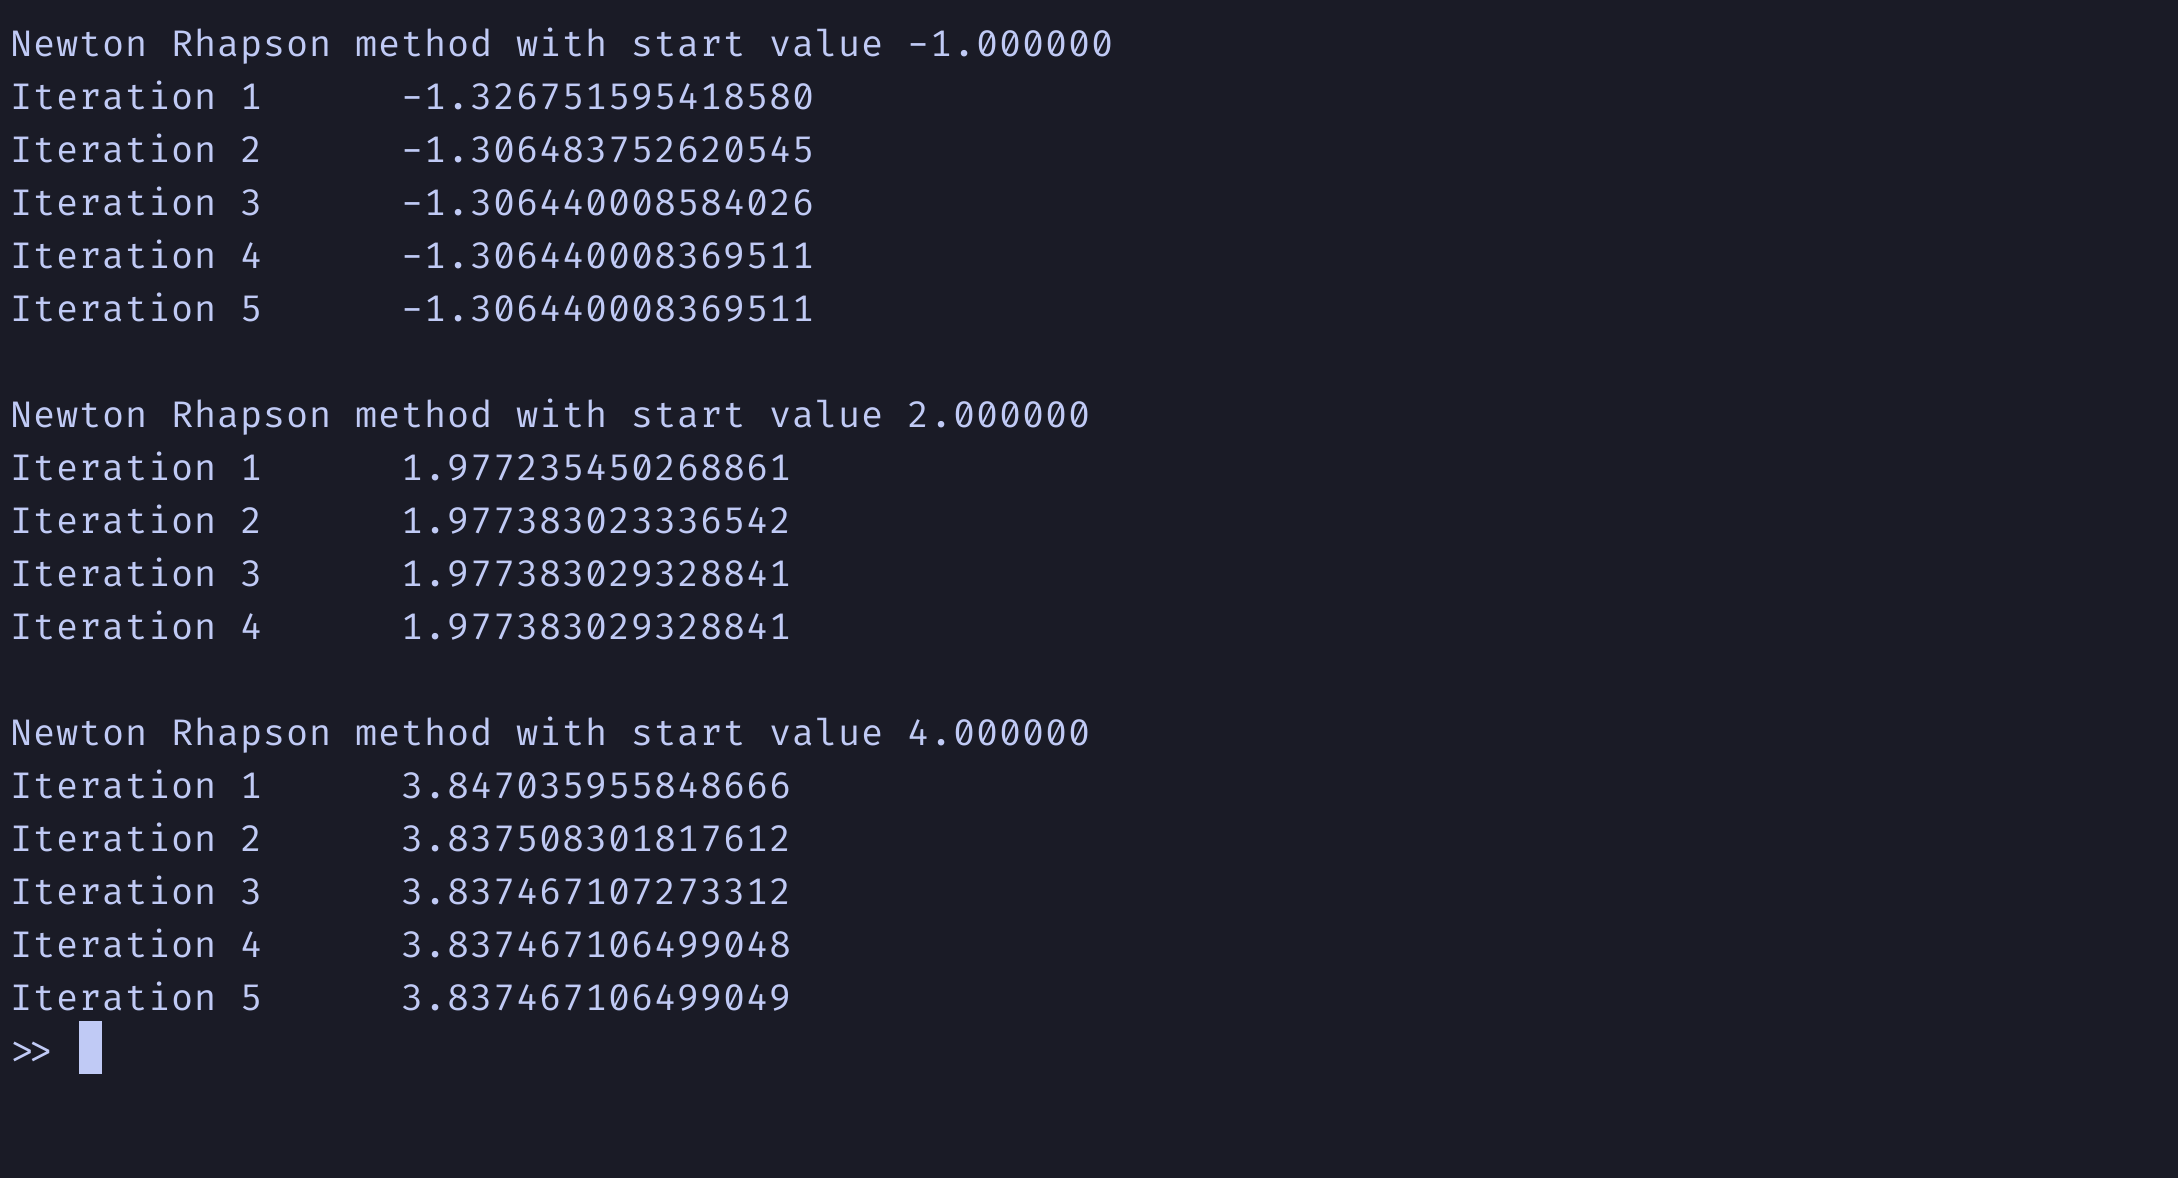
\includegraphics[width=0.8\textwidth]{imgs/q6_results.png}
	\caption{Results for question 6}
	\label{fig:q6_result}
\end{figure}
The Newton Rhapson method does not converge if the derivative at the given point is 0. An initial value of 3 is not an appropriate basin of attraction, this consequently caused the script to repeat indefinetly, as opposed to converging. 

Roughly 5 interations were required to reach each root when the methods tolerance was set to $10^{-15}$. Other tolerances were tested, though not included as they were deemed inconsequential.
\newpage
\section{}
\begin{figure}[H]
	\centering
	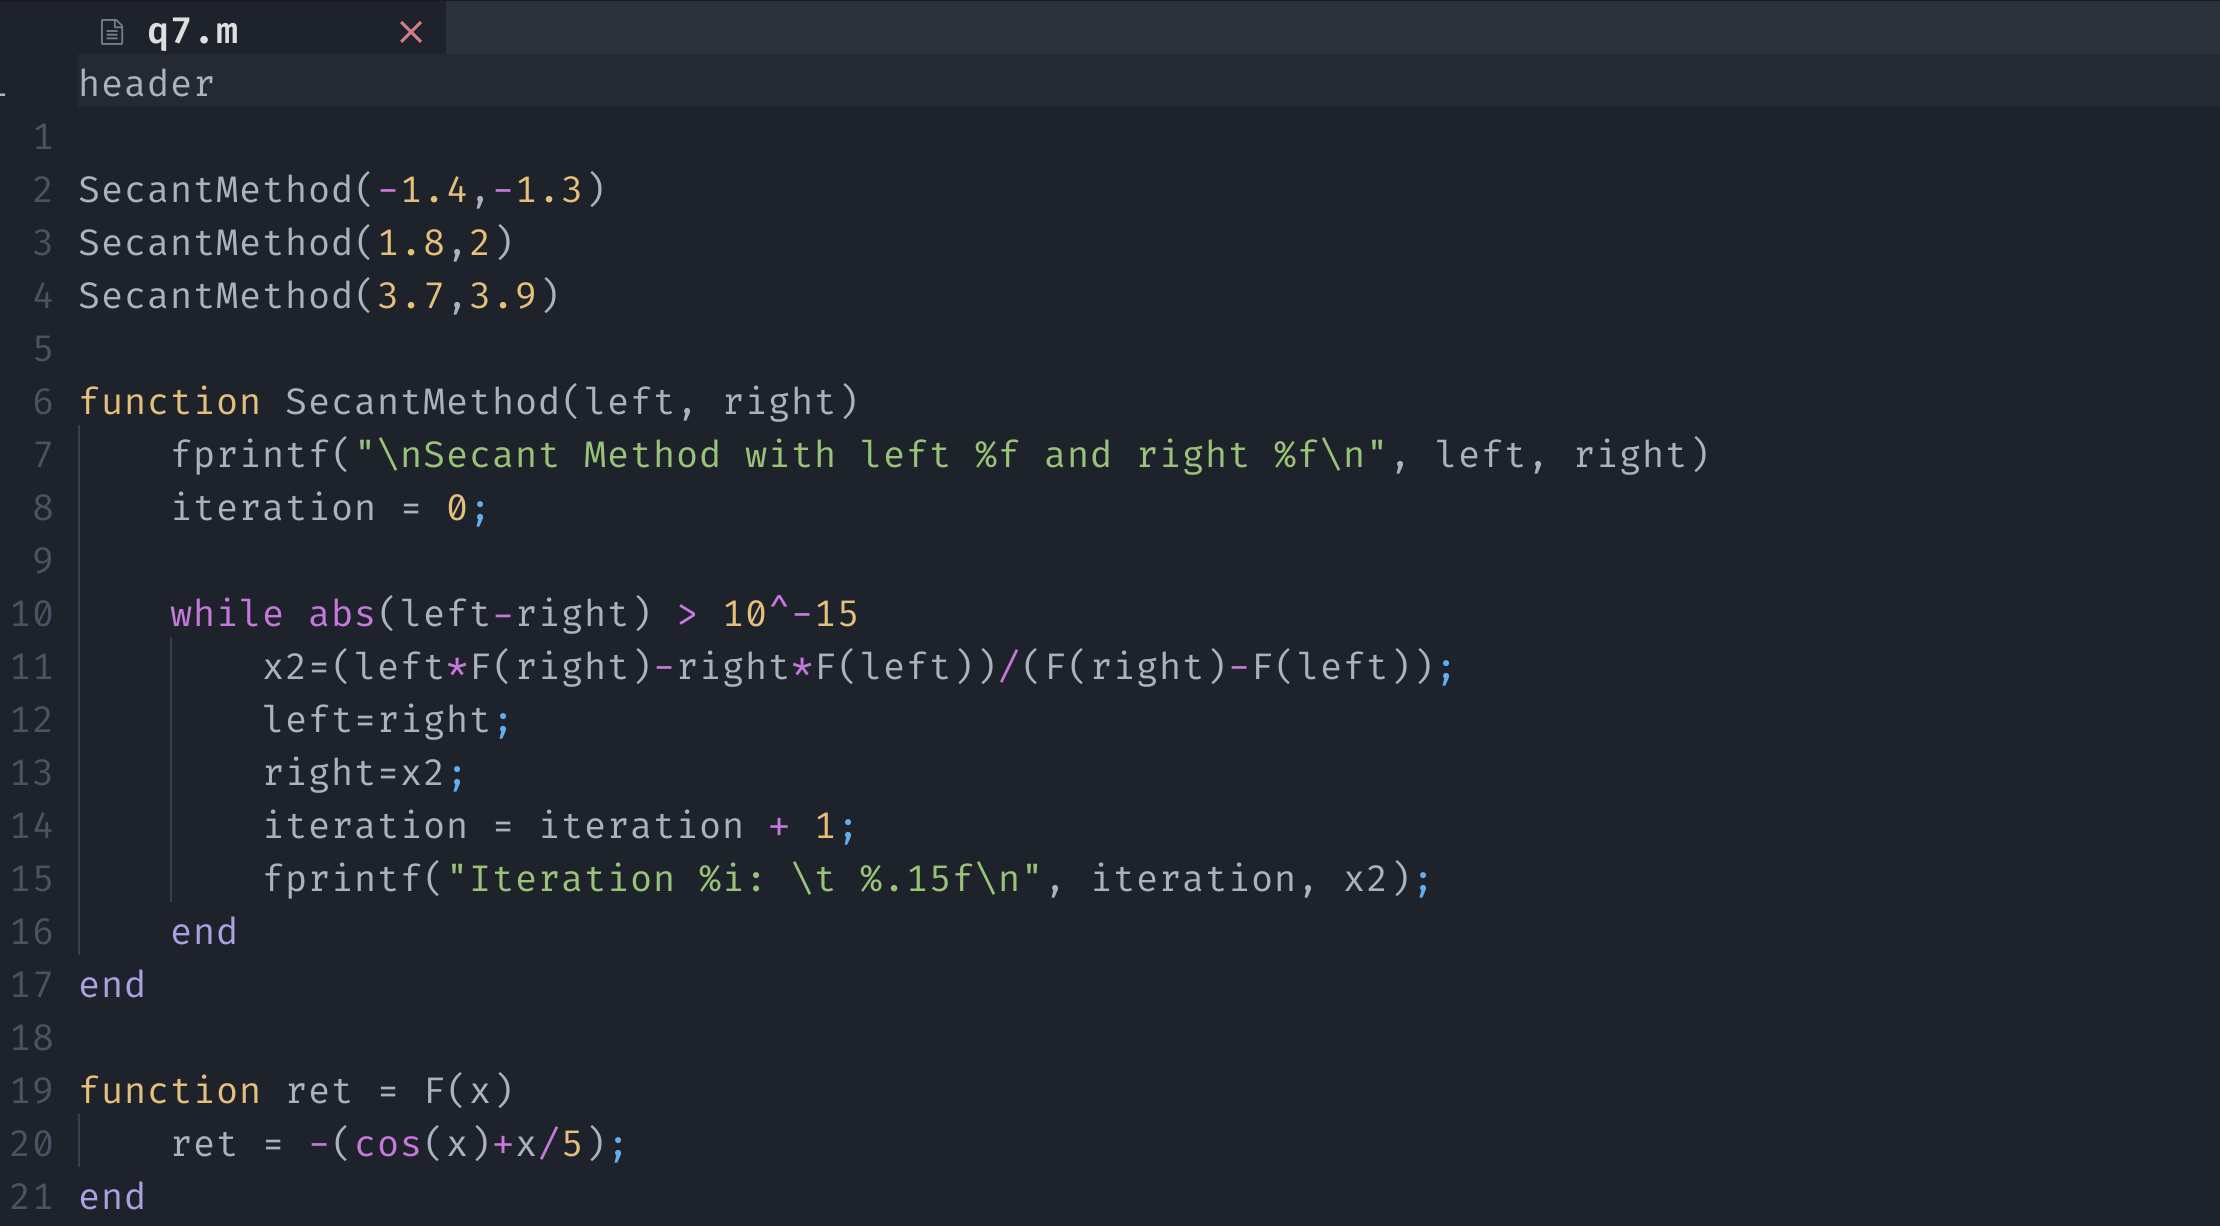
\includegraphics[width=0.8\textwidth]{imgs/q7_code.png}
	\caption{Code for question 7}
	\label{fig:q7_code}
\end{figure}

\begin{figure}[H]
	\centering
	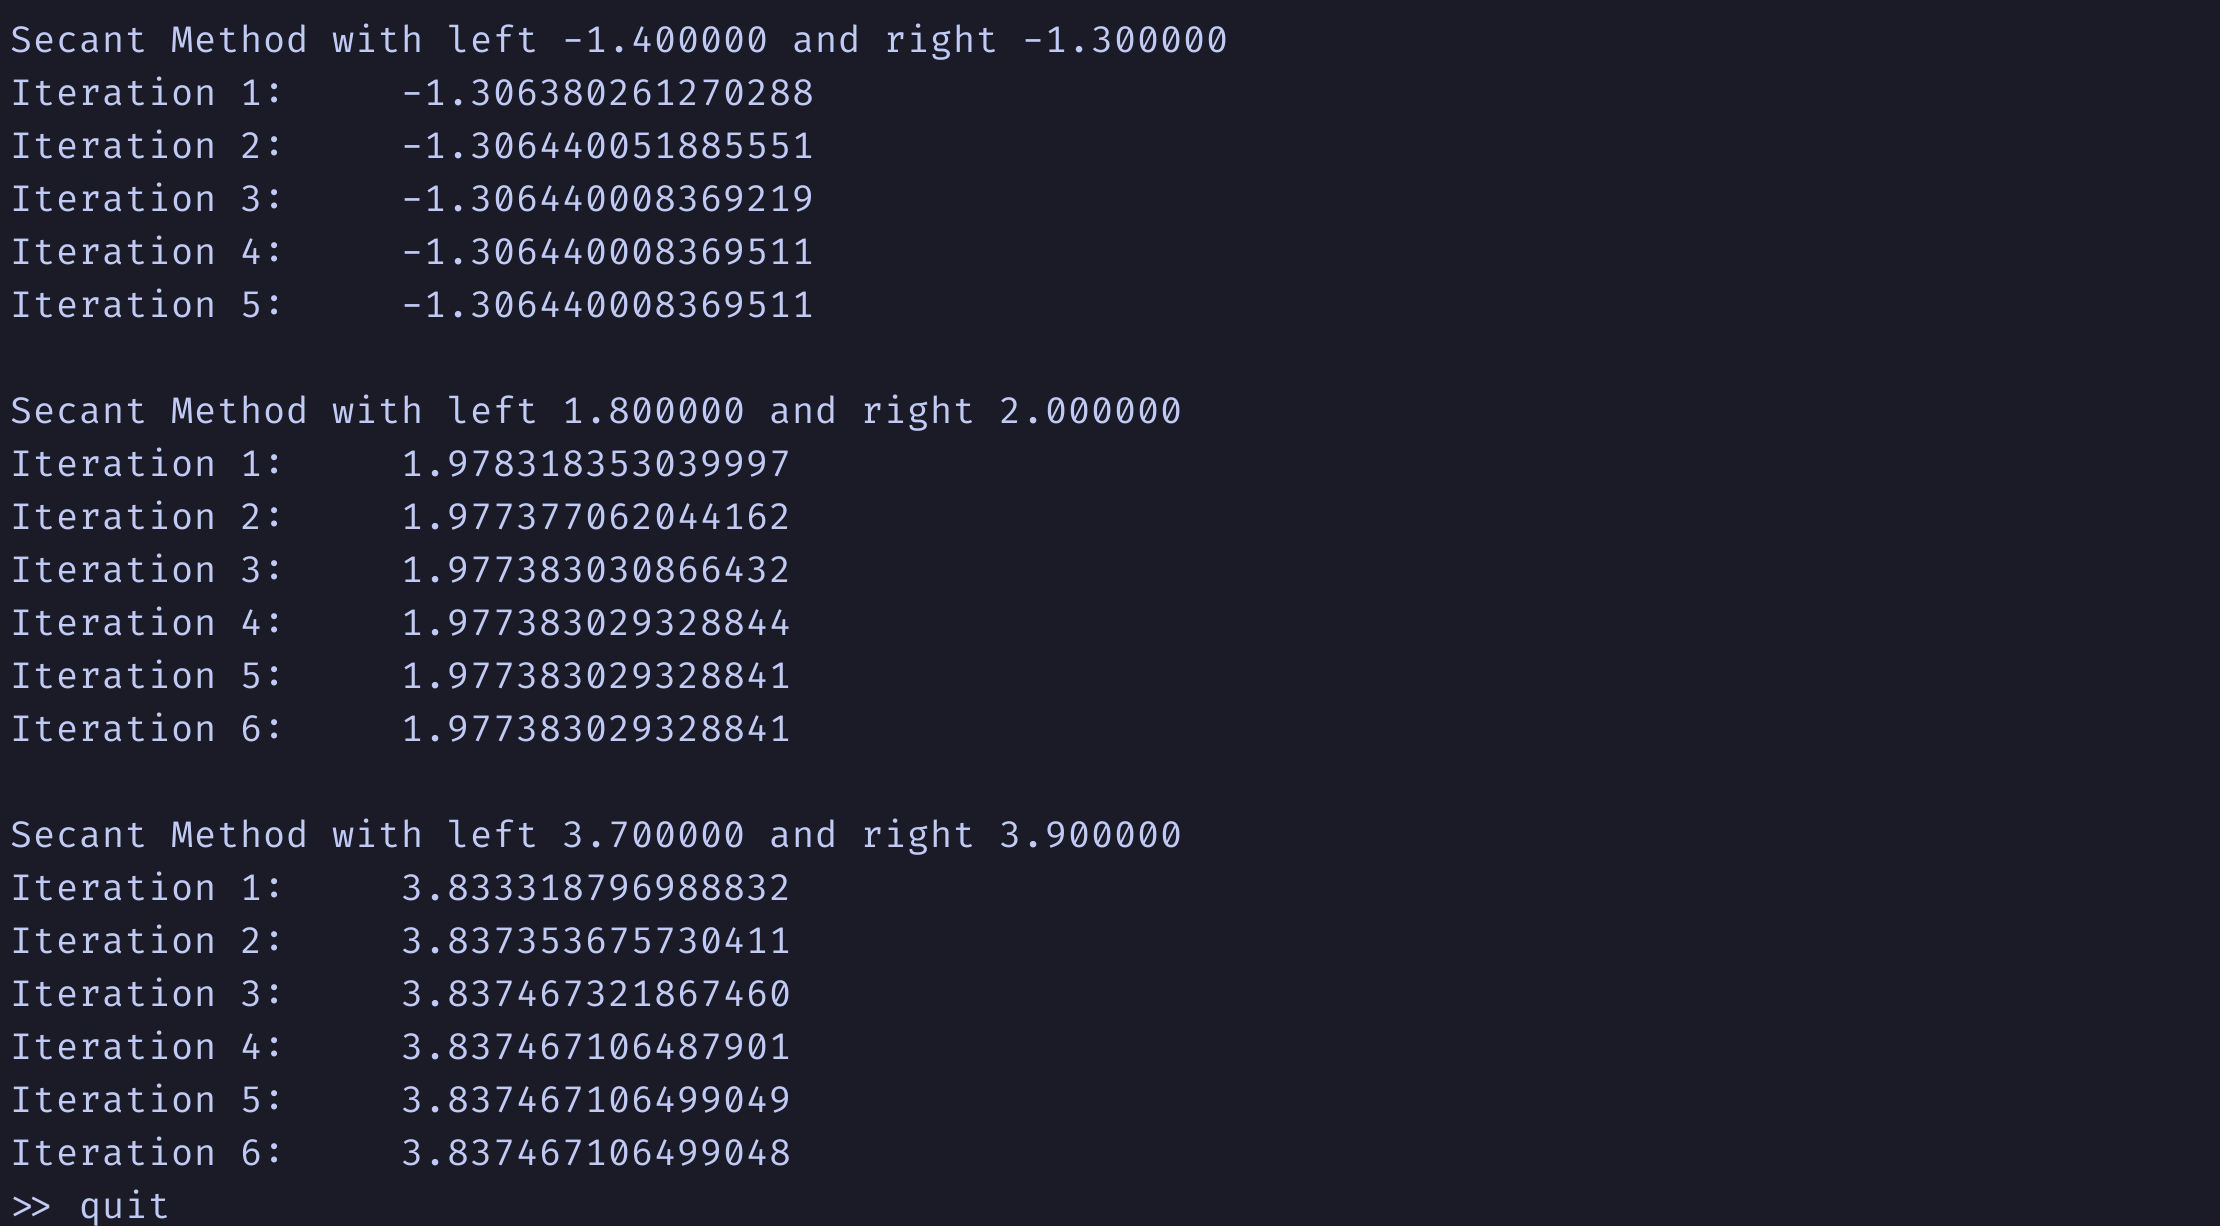
\includegraphics[width=0.8\textwidth]{imgs/q7_results.png}
	\caption{Results for question 7}
	\label{fig:q7_result}
\end{figure}
The Secant method requires more iterations to converge as opposed to the Newton Rhapson method, this evidently means that the Newton Rhapson method will generally converge quicker.

The notable difference between either functions is that the Secant method only requires the function and two starting values. The Newton Rhapson method on the other hand requires only one starting value, but does also require the functions derivative. 
\newpage
\section{}

\begin{figure}[H]
	\centering
	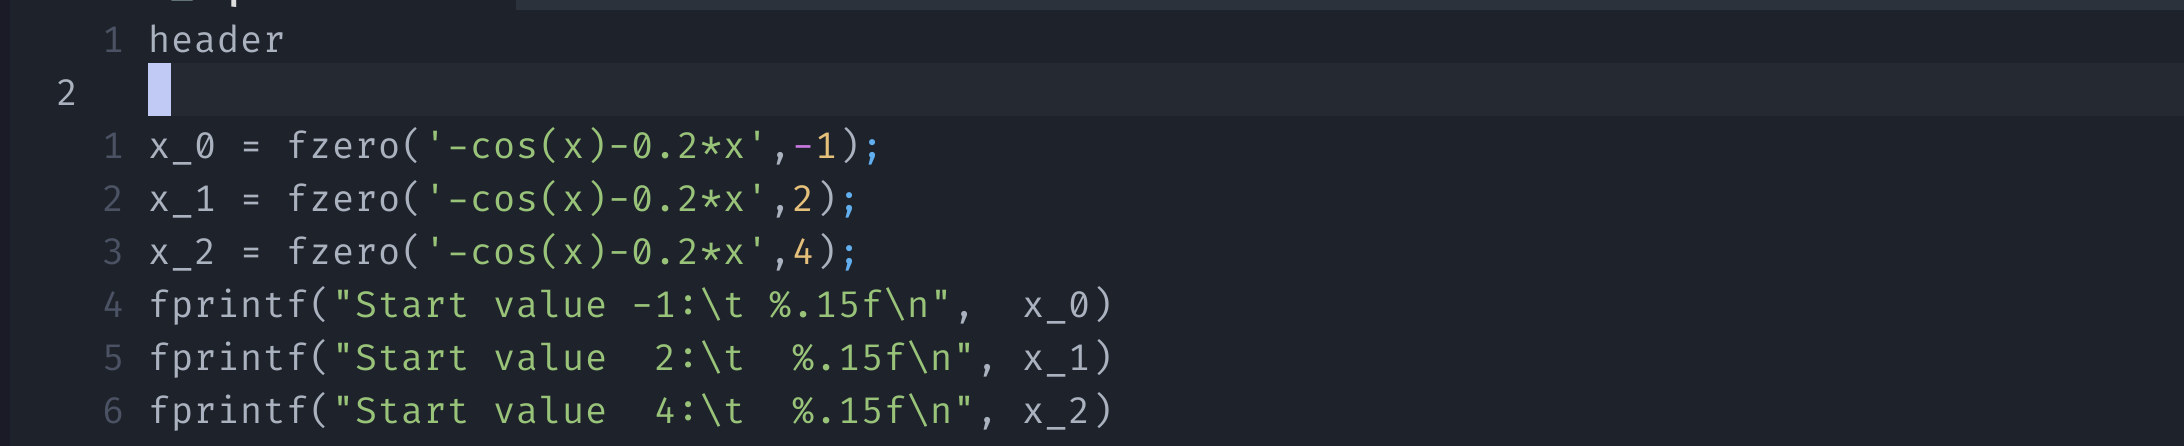
\includegraphics[width=0.8\textwidth]{imgs/q8_code.png}
	\caption{Code for question 8}
	\label{fig:q8_code}
\end{figure}

\begin{figure}[H]
	\centering
	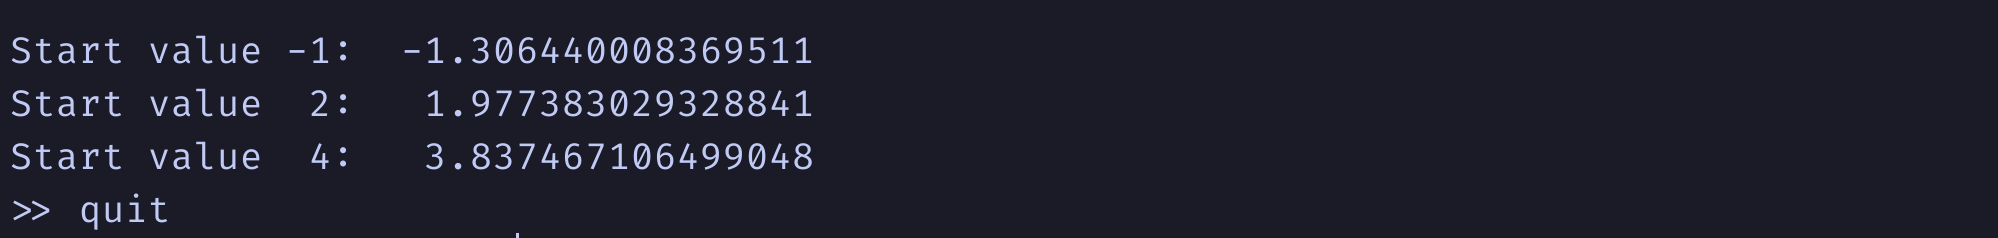
\includegraphics[width=0.8\textwidth]{imgs/q8_results.png}
	\caption{Results for question 8}
	\label{fig:q8_result}
\end{figure}






\end{document}
